\documentclass{minimal}

\usepackage{tikz}
\usepackage{pgfplots}
\usetikzlibrary{positioning}
\usetikzlibrary{arrows}
\usetikzlibrary{patterns}
\usepackage{tikz-dimline}
\usepackage{amsmath}
\tikzset{every picture/.append style={font=\large}}
% \usepackage{mathpazo}



\begin{document}

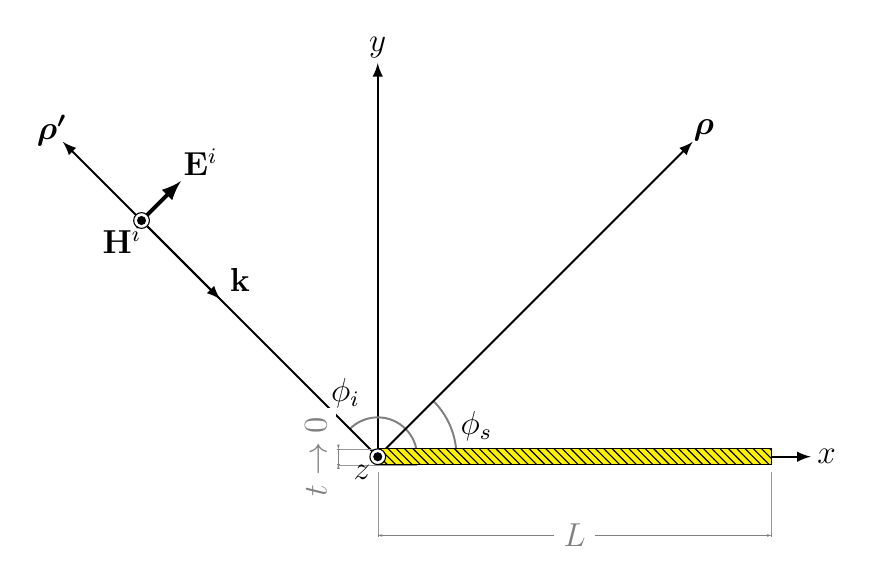
\begin{tikzpicture}
  % % Draw coordinate system
  % Axes
  % z-axis
  % \draw [color=black, fill=black] (0, 0) circle (0.1);
  % \draw [color=black, fill=none] (0, 0) circle (0.2);
  % x-axis
  \draw [line width=0.25mm,arrows={-latex}] (0, 0) -- (5.5, 0);
  % y-axis
  \draw [line width=0.25mm,arrows={-latex}] (0, 0) -- (0, 5);

  % Axis Labels
  % x-axis label
  \node at (5.7, 0) {$x$};
  % y-axis label
  \node at (0, 5.2) {$y$};

% % Normal Vector n
% \draw [line width=0.5mm,arrows={-latex}] (0, 0) -- (0, 1)
% node [near end, above right,black] {$\boldmath{\hat n}$};;



  % Draw Angle Arcs
  % Observation Angle
  \draw [gray,line width=0.25mm] (1.0,0) arc [start angle=0, end angle=45, radius=1cm]
  node [midway, right,black] {$\phi_s$};

  % Source Angle
  \draw [gray,line width=0.25mm] (.5,0) arc [start angle=0, end angle=135, radius=.5cm]
  node [near end, above left,black] {$\phi_i$};

  % Source and Observation points
  % Observation Coordinates
  % p
  \draw [line width=0.25mm,arrows={-latex}] (0, 0) -- (4, 4);
  % p label
  \node at (4.14, 4.14) {$\boldsymbol{\rho}$};

  % Source Point
  % p'
  \draw [line width=0.25mm,arrows={-latex}] (0, 0) -- (-4, 4);

  % p' label
  \node at (-4.14, 4.14) {$\boldsymbol{\rho'}$};

  % Field Specs

  % Draw k-vector
  \draw [line width=0.25mm,arrows={-latex}] (-3, 3) -- (-2, 2);
  \node at (-1.75, 2.25) {$\mathbf{k}$};

  % Draw E-field
  \draw [line width=0.5mm,arrows={-latex}] (-3, 3) -- (-2.5, 3.5);
  \node at (-2.25, 3.74) {$\mathbf{E}^i$};

  % Draw H-field
  \draw [color=black, fill=white] (-3, 3) circle (0.1);
  \draw [color=black, fill=black] (-3, 3) circle (0.05);
  \node at (-3.25, 2.75) {$\mathbf{H}^i$};

  % Draw Dimension
  \dimline[line style = {gray, line width=0.2},
  extension start length=-.16,
  extension end length=-.16] {(0,-1)}{(5, -1)}{$L$};

  \dimline[line style = {gray, line width=0.2,
  arrows=dimline reverse-dimline reverse},label style={above=0.2ex},
  ] {(-.5,-.1)}{(-.5, .1)}{$t \to 0$};

  % Draw plate
  % \draw [line width=1mm,color=gray] (-2.5, 0) -- (2.5, 0);
  \draw[fill=yellow]  (0,-.1) rectangle (5,.1);

  % Draw plate
  \draw[pattern=north west lines, pattern color=black]  (0,-.1) rectangle (5,.1);

  % z-axis label
  \draw [color=black, fill=white] (-0, 0) circle (0.1);
  \draw [color=black, fill=black] (-0, 0) circle (0.05);
  \node at (-.2, -.2) {$z$};
  
\end{tikzpicture}
\end{document}
